% toy-lecture.tex — 5-frame fixture deck for /compile-latex, /translate-to-quarto,
% /qa-quarto, and /extract-tikz testing (Workstream B-II; see tests/TESTING.md).
% Deliberately SELF-CONTAINED: no house preamble, so it compiles from this
% directory with plain `xelatex toy-lecture` (3-pass + bibtex).
\documentclass[11pt]{beamer}
\usetheme{default}
\usecolortheme{seahorse}
\usepackage{amsmath}
\usepackage{natbib}
\usepackage{tikz}
\usetikzlibrary{positioning, arrows.meta}

% Minimal stand-in for the house `keybox` environment (kept dependency-free).
\newenvironment{keybox}%
  {\begin{beamercolorbox}[rounded=true, sep=6pt]{block body example}}%
  {\end{beamercolorbox}}

\title{Difference-in-Differences on the Toy Panel}
\subtitle{A five-frame fixture deck}
\author{Workflow Test Bed}
\date{June 2026}

\begin{document}

% --- Frame 1: title ---------------------------------------------------
\begin{frame}
  \titlepage
\end{frame}

% --- Frame 2: motivation (citation) -----------------------------------
\begin{frame}{Why a known DGP?}
  \begin{itemize}
    \item A reviewer that has never caught a planted bug is untested.
    \item The toy panel hardcodes its treatment effect, so every estimate downstream has a ground truth.
    \item Staggered-adoption pitfalls are deliberately absent here: common timing keeps two-way fixed effects clean \citep{goodmanbacon2021}.
    \item Heterogeneity-robust estimators are exercised elsewhere \citep{callaway2021}.
  \end{itemize}
\end{frame}

% --- Frame 3: estimand (equation + box) --------------------------------
\begin{frame}{The estimand}
  The fixture outcome follows
  \begin{equation}
    y_{it} = \alpha_i + \gamma_t + \tau \, D_{it} + \varepsilon_{it},
    \qquad \varepsilon_{it} \sim \mathcal{N}(0, 1),
    \label{eq:dgp}
  \end{equation}
  with $D_{it} = \mathbf{1}\{i \text{ treated}\} \cdot \mathbf{1}\{t \ge 2015\}$.

  \begin{keybox}
    \textbf{Key point.} The true effect is $\tau = 2$ by construction; the
    seeded reference estimate is $\hat{\tau} = 1.71$ (cluster SE $0.37$).
  \end{keybox}
\end{frame}

% --- Frame 4: TikZ figure ----------------------------------------------
\begin{frame}{Design timeline}
  \begin{center}
    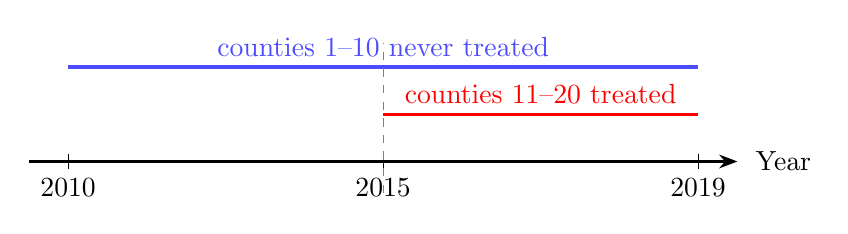
\begin{tikzpicture}[>=Stealth, node distance=6mm]
      \draw[->, thick] (0,0) -- (9,0) node[right=1mm] {Year};
      \foreach \x/\yr in {0.5/2010, 4.5/2015, 8.5/2019} {
        \draw (\x,0.1) -- (\x,-0.1) node[below] {\yr};
      }
      \draw[very thick, red] (4.5,0.6) -- (8.5,0.6)
        node[above, pos=0.5, red] {counties 11--20 treated};
      \draw[very thick, blue!70] (0.5,1.2) -- (8.5,1.2)
        node[above, pos=0.5, blue!70] {counties 1--10 never treated};
      \draw[dashed, gray] (4.5,-0.4) -- (4.5,1.5);
    \end{tikzpicture}
  \end{center}
\end{frame}

% --- Frame 5: summary + references --------------------------------------
\begin{frame}{Summary}
  \begin{itemize}
    \item Equation~\eqref{eq:dgp} is the single source of truth for every test.
    \item Balanced panel: 20 counties $\times$ 10 years $= 200$ observations.
    \item Regenerate with \texttt{make\_fixtures.py} (seeded).
  \end{itemize}
  \vfill
  \bibliographystyle{plainnat}
  \bibliography{toy-lecture}
\end{frame}

\end{document}
